\documentclass{beamer}
\usepackage[T1]{fontenc}
\usepackage[utf8]{inputenc}
\usepackage{lmodern}
\usepackage[francais]{babel}
\usepackage{graphicx}
\usepackage{beamerthemeWarsaw}
\expandafter\def\expandafter\insertshorttitle\expandafter{\insertshorttitle\hfill\insertframenumber\,/\,\inserttotalframenumber}

\title{Des réseaux et des drones}
\author{Olivier \bsc{Boissard}, Kevin \bsc{Boulala}}
\institute{Université de Franche Comté}
\date{\today}

\begin{document}

\begin{frame}
  \titlepage
\end{frame}

\begin{frame}
	\tableofcontents[]
\end{frame}

\section{Les drones}
\subsection{Définition}
\begin{frame}
  \frametitle{C'est large quand même}
  %TODO
  \begin{block}{Todo}
    Un drone, ça peut être beaucoup de choses.
  \end{block}
\end{frame}

\begin{frame}
  \frametitle{Taille, forme}
  %TODO
  \begin{block}{Todo}
    Quelques informations sur ce qui existe.
  \end{block}
\end{frame}

\subsection{Rapidement, quelle utilité ?}
\begin{frame}
  \frametitle{Militaire, civil}
  %TODO
  \begin{block}{Todo}
    Un court historique de l'utilité des drones.
  \end{block}
\end{frame}

\section{Des réseaux et des drones}
\begin{frame}
	\tableofcontents[currentsection]
\end{frame}

\subsection{Aquila}
\begin{frame}
  \frametitle{Le projet de Facebook}
  \begin{alertblock}{Avertissement}
    Facebook parle beaucoup pour faire rêver mais peu de technique dans son discours !
  \end{alertblock}
  %TODO
  \begin{block}{Todo}
    Qu'est ce qu'ils font ? Pourquoi ils le font ?
  \end{block}
\end{frame}

\begin{frame}
  \frametitle{Sacré engin}
  %TODO
  \begin{block}{Cheese}
      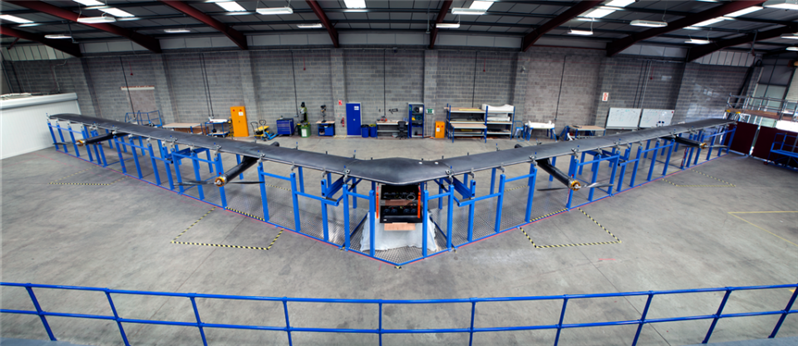
\includegraphics[width=\textwidth]{../Images/facebook_aquila.png}
  \end{block}
\end{frame}

\end{document}
